\documentclass[10pt, a4paper]{article} % use larger type; default would be 10pt

\usepackage{fontspec} % Font selection for XeLaTeX; see fontspec.pdf for documentation
\defaultfontfeatures{Mapping=tex-text} % to support TeX conventions like ``---''
\usepackage{xunicode} % Unicode support for LaTeX character names (accents, European chars, etc)
\usepackage{xltxtra} % Extra customizations for XeLaTeX
\usepackage{tikz}
% \usepackage{coloremoji}
\usetikzlibrary{arrows,calc,patterns}


% other LaTeX packages.....
\usepackage{fullpage}
\usepackage[top=2cm, bottom=4.5cm, left=2.5cm, right=2.5cm]{geometry}
\usepackage{amsmath,amsthm,amsfonts,amssymb,amscd,systeme}
\usepackage{unicode-math}
\usepackage{cancel}
\geometry{a4paper} 
\usepackage[parfill]{parskip} % Activate to begin paragraphs with an empty line rather than an indent
\usepackage{fancyhdr}
\usepackage{listings}
\usepackage{graphicx}
\usepackage{hyperref}
\usepackage{multicol}

\usepackage{xcolor}

% FONTS
% \setmainfont[Ligatures=TeX]{Cambria Math} % set the main body font (\textrm), assumes Charis SIL is installed
%\setsansfont{Deja Vu Sans}
% \setmonofont[Ligatures=TeX]{Fira Code}
\setmathfont[Ligatures=TeX]{NewCMMath-Regular}

\setmainfont{Cambria}
\setmonofont[Ligatures=TeX]{Roboto Mono}

\renewcommand\lstlistingname{Algorithm}
\renewcommand\lstlistlistingname{Algorithms}
\def\lstlistingautorefname{Alg.}
\lstdefinestyle{mystyle}{
    % backgroundcolor=\color{backcolour},   
    % commentstyle=\color{codegreen},
    % keywordstyle=\color{magenta},
    % numberstyle=\tiny\color{codegray},
    % stringstyle=\color{codepurple},
    basicstyle=\ttfamily\footnotesize,
    breakatwhitespace=false,         
    breaklines=true,                 
    captionpos=b,                    
    keepspaces=true,                 
    numbers=left,                    
    numbersep=5pt,                  
    showspaces=false,                
    showstringspaces=false,
    showtabs=false,                  
    tabsize=2
}
\lstset{style=mystyle}

\newcommand\course{MS2 - Алгебри Лі}
\newcommand\hwnumber{Модуль 1}                   % <-- homework number
\newcommand\idgroup{111-2023}                
\newcommand\idname{Михайло Корешков}  

\usepackage[framemethod=TikZ]{mdframed}
\mdfsetup{%
	backgroundcolor = black!5,
    skipabove = 4pt,
}
\mdfdefinestyle{ans}{%
    backgroundcolor = green!5,
    linecolor = green!50,
    linewidth = 1pt,
}

\pagestyle{fancyplain}
\headheight 35pt
\lhead{\idgroup \\ \idname}
\chead{\textbf{\Large \hwnumber}}
\rhead{\course \\ \today}
\lfoot{}
\cfoot{}
\rfoot{\small\thepage}
\headsep 1.5em

\linespread{1.2}

\newcommand{\R}{\mathbb{R}}
\newcommand{\N}{\mathbb{N}}
\newcommand{\Z}{\mathbb{Z}}
\newcommand{\J}{J}
\DeclareMathOperator{\lcm}{lcm}
\DeclareMathOperator{\cd}{CD}
\DeclareMathOperator{\id}{id}
\DeclareMathOperator{\rank}{rank}

\newcommand{\g}{\mathfrak{g}}

\renewcommand{\B}{\mathcal{B}}

\newtheorem*{definition}{Визначення}

\newcommand{\todo}[1]{\colorbox{red}{\textbf{TODO}: #1}}


\begin{document}

\section*{№1}

\begin{mdframed}
    Знайти центр алгебри \quad
    $\g = \g_{6.6} : [e_1,e_2]=e_4, [e_2,e_3]=e_6, [e_2,e_4]=e_5$
\end{mdframed}

Розглянемо загальний випадок комутатора в цій алгебрі.
Нехай $x,y \in \g$ та $x = \sum_{i=1}^6 x_ie_i, y = \sum_{j=1}^6 y_je_j$.

\begin{align} \label{eq:1.1}    
    [x,y] &= ( x_1y_2-x_2y_1 ) e_4  + ( x_2y_3 - x_3y_2 ) e_6 + ( x_2y_4 - x_4y_2 ) e_5
\end{align}

$I$ - ідеал алгебри $\g$ якщо $\forall x \in I, y \in \g: [x,y] \in I$.\\
Центр алгебри $Z(\g)$ визначається як $Z(\g) = \{x \in \g \mid \forall y \in \g: [x,y] = 0\}$.\\
Центр є лінійним підпростором. 
Дійсно, для $u,v\in Z(\g)$ маємо $\forall a,b \in \mathbb{F}, y\in\g: [(au+bv),y] = a[u,y] + b[v,y] = 0$,
тобто $(au+bv) \in Z(\g)$.\\
Центр є ідеалом:
$u \in Z(\g) \implies \forall y\in\g: [u,y] = 0 \in Z(\g)$.

Зверну увагу, що змінні $x_5, x_6$ не входять у рівняння \ref{eq:1.1}.
Нехай $x = x_5e_5 + x_6e_6$, тобто $x_1=x_2=x_3=x_4=0$. Тоді $\forall y: [x,y] = 0$.
Отже, 
\[<e_5, e_6> \subset Z(\g)\]

Далі, для $x\in Z(\g)$ з рівняння \ref{eq:1.1} маємо наступні співвідношення
\begin{equation} \label{eq:1.2}
    \forall y \in \g: \quad \begin{vmatrix}
        x_1 & x_2 \\ y_1 & y_2
    \end{vmatrix} =
    \begin{vmatrix}
        x_2 & x_3 \\ y_2 & y_3
    \end{vmatrix} =  
    \begin{vmatrix}
        x_2 & x_4 \\ y_2 & y_4
    \end{vmatrix} = 0.
\end{equation}

Покладемо $x = \sum_{i=1}^6 \in Z(\g)$ та $V = <e_1,e_2,e_3,e_4>, \dim V = 4$.\\
Припустимо, що $x \notin <e_5,e_6>$.\\
Тоді $x' = (x - x_5e_5 - x_6e_6) \in Z(\g) \cap V$ 
(бо $<e_5, e_6> \subset Z(\g)$, $Z(\g)$ - лінійна множина, та $x' \in V$).
При цьому з припущення маємо $x' \ne 0$. 
Тоді можна взяти інший базис $V = <x',v_1,v_2,v_3>$.
З \ref{eq:1.2} маємо що $\forall y \in V: \exists k: y=kx$.
Але тоді $\exists k: v_1 = kx'$, звідки $\dim V < 4$. Отримали суперечність. \\
Отже, $x \in <e_5,e_6>$.

Тобто, \colorbox{green}{$Z(\g) = <e_5, e_6>$}

\newpage
\section*{№2}
\begin{mdframed}
    Побудувати оператори приєднаного диференціювання для алгебри ($a \ge 0$)
    \[\g : [e_2,e_3]=e_1,\; [e_1,e_4]=2ae_1,\; [e_2,e_4]=ae_2-e_3,\; [e_3,e_4]=e_2+ae_3.\]
\end{mdframed}

Обчислимо структурні сталі $C_{ij}^k$.
\[[e_i, e_j] = \sum_{k} C_{ij}^k e_k\]
\[C_{23}^1 = -C_{32}^1 = 1, \quad C_{14}^1 = -C_{41}^1 = 2a, \quad C_{24}^2 = -C_{42}^2 = a;\]
\[C_{24}^3 = -C_{42}^3 = -1, \quad C_{34}^2 = -C_{43}^2 = 1, \quad C_{34}^3 = -C_{43}^3 = a.\]
Всі інші нулі.

\[ad_{e_k} x = [e_k, x] = \sum_{i} x_i[e_k,e_i] = \sum_{ij} x_i C_{ki}^j e_j\]
\[(ad_{e_k} x)_l = \sum_{i} x_i C_{ki}^l\]
Тобто матриці операторів $ad_{e_k}$ визначаються як $(ad_{e_k})_{ij} = C_{kj}^i$.

\[ad_{e_1} = (C_{1j}^i) = \begin{pmatrix}
    0 & 0 & 0 & 2a\\
    0 & 0 & 0 & 0\\
    0 & 0 & 0 & 0\\
    0 & 0 & 0 & 0
\end{pmatrix} \quad
ad_{e_2} = (C_{2j}^i) = \begin{pmatrix}
    0 & 0 & 1 & 0\\
    0 & 0 & 0 & a\\
    0 & 0 & 0 & -1\\
    0 & 0 & 0 & 0
\end{pmatrix}\]
\[ad_{e_3} = (C_{3j}^i) = \begin{pmatrix}
    0 & -1 & 0 & 0\\
    0 & 0 & 0 & 1\\
    0 & 0 & 0 & a\\
    0 & 0 & 0 & 0
\end{pmatrix} \quad
ad_{e_4} = (C_{4j}^i) = \begin{pmatrix}
    -2a & 0 & 0 & 0\\
    0 & -a & -1 & 0\\
    0 & +1 & -a & 0\\
    0 & 0 & 0 & 0
\end{pmatrix}\]

\newpage
\section*{№3}
\begin{mdframed}
    Знайти комутаційні співвідношення. $\lambda \in \mathbb R$.
    \[a_1 = \partial_1\]
    \[a_2 = x_2\partial_1 + x_3\partial_2\]
    \[a_3 = \partial_2\]
    \[a_4 = (2\lambda x_1 - \frac{1}{2}x_2^2)\partial_1 + (\lambda-x_3)x_2\partial_2 - (1+x_3^2)\partial_3\]
\end{mdframed}

Комутаційні співвідношення визначаються як $[x,y]f = x(y(f)) - y(x(f))$.
Диференціали другого порядку зникнуть через достатню гладкість всіх коефіцієнтів. 

\[ [a_1, a_2] = \cancelto{0}{\partial_1(x_2)}\partial_1+\cancelto{0}{\partial_1(x_3)}\partial_2 - x_2\cancelto{0}{\partial_1(1)}\partial_1 - x_3\cancelto{0}{\partial_2(1)}\partial_1 = 0\]
\[ [a_1, a_3] = \partial_1\partial_3 - \partial_3\partial_1 = 0\]
\begin{align*}
    [a_1, a_4] &= \partial_1(2\lambda x_1 - \frac{1}{2}x_2^2)\partial_1 + \cancelto{0}{\partial_1((\lambda-x_3)x_2)}\partial_2 - \cancelto{0}{\partial_1(1+x_3^2)}\partial_3 - \\
    &- \left(...\partial_1(1)\partial_1 + ...\partial_2(1)\partial_1 + ...\partial_3(1)\partial_1\right) = \\
    &= 2\lambda\partial_1 = 2 \lambda a_1
\end{align*}
\[ [a_2, a_3] = -1 \cdot \partial_1 = -a_1\]
\[ [a_2, a_4] = \lambda x_{2} \partial_1 + \lambda x_{3} \partial_2 + \partial_{2} = \lambda a_2 + a_3\]
\[ [a_3, a_4] = \lambda \partial_2 - x_{2} \partial_1 - x_{3} \partial_2 = \lambda a_3 - a_2 \]

Перевірив за допомогою бібліотеки символьних обчислень для Python

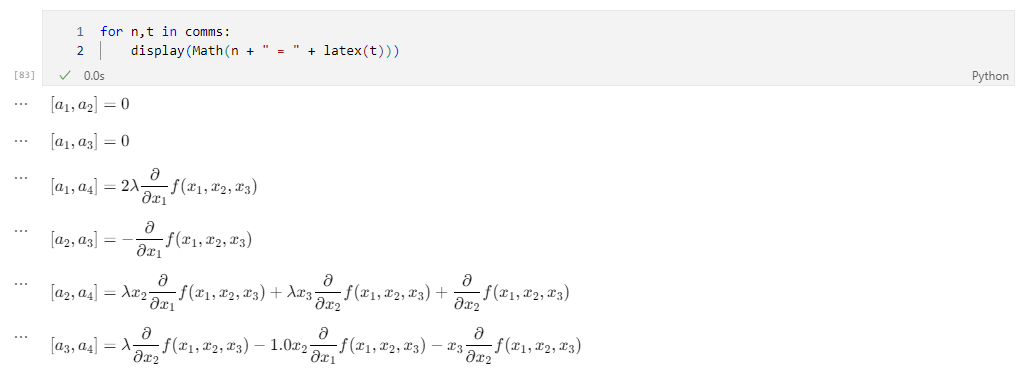
\includegraphics[width=\textwidth]{1.png}

Тобто 
\[\g : [a_1, a_4] = 2\lambda a_1; \quad [a_2, a_3] = -a_1; \quad [a_2, a_4] = \lambda a_2 + a_3; \quad [a_3, a_4] = \lambda a_3 - a_2. \]

$[a_2+\lambda a_3,a_4] = \lambda a_2 + a_3 + \lambda^2 a_3 - \lambda a_2 = (1+\lambda^2) a_3$\\
$[a_3-\lambda a_2, a_4] = \lambda a_3 - a_2 - \lambda^2 a_2 - \lambda a_3 = -(1+\lambda^2) a_2$

Тобто $\g' = <a_1, a_2, a_3>$.

Не знаю що це за алгебра :(

\section*{№4}

\begin{mdframed}
    Дослідити на нільпотентність та розв'язність
    \[\g = \g_{5.6} : [e_1,e_2] = e_3, \quad [e_1,e_3]=e_4, \quad [e_1,e_4]=e_5, \quad [e_2,e_3]=e_5.\]
\end{mdframed}

$\g^2 = \g' = [\g,\g] = <e_3,e_4,e_5>$ - з правого боку комутаційних співвідношень.

$\g^3 = [\g, \g^2] = <[e_1,e_3],[e_1,e_4],[e_1,e_5],[e_2,e_3],[e_2,e_4],[e_2,e_5],[e_3,e_4],[e_3,e_5],[e_4,e_5]> = $\\
$= <e_4, e_5, 0, e_5, 0, 0, 0, 0, 0> = <e_4,e_5>$

$\g^4 = [\g, \g^3] = <[e_1,e_4],[e_1,e_5],[e_2,e_4],[e_2,e_5],[e_3,e_4],[e_3,e_5],[e_4,e_5]> = $\\
$= <e_5,0,0,0,0,0,0> = <e_5>$

$\g^5 = [\g, \g^4] = <[e_1,e_5],[e_2,e_5],[e_3,e_5],[e_4,e_5]> = <0,0,0,0> = 0$

Отже, алгебра \colorbox{green}{нільпотентна}. Звідси маємо, що вона і \colorbox{green}{розв'язна}.

Дійсно
$\g'' = [\g',\g'] = <[e_3,e_4],[e_3,e_5],[e_4,e_5]> = <0,0,0> = 0$


\section*{№5}
\begin{mdframed}
    $\g : [e_1,e_2] = e_1, \quad [e_3,e_4]=e_3$.
    Знайти першу та другу похідні. Перевірити ізоморфність із $\mathfrak{sl}(2,\R)\oplus \g_1$.
\end{mdframed}

$g' = [\g, \g] = <e_1,e_3>$ - з правого боку комутаційних співвідношень.

$g'' = [\g',\g'] = <[e_1,e_3]> = 0$

Тобто, алгебра \colorbox{green}{розв'язна}.

При цьому 
$[\g, \g^2] = <[e_1,e_3],[e_2,e_1],[e_2,e_3],[e_4,e_1],[e_4,e_3]> = <e_1,e_3> = \g^2$.\\
Отже, алгебра \colorbox{green}{не нільпотентна}.

Припустимо, що $x \in Z(\g)$.
\[[x,y] = (x_1y_2-x_2y_1)e_1 + (x_3y_4-x_4y_3)e_3 = 0\]
\[\begin{vmatrix}
    x_1 & x_2 \\ y_1 & y_2
\end{vmatrix} = \begin{vmatrix}
    x_3 & x_4 \\ y_3 & y_4
\end{vmatrix} = 0\]
\[\forall y: \begin{cases}
    x_1 = k_1 y_1\\
    x_2 = k_1 y_2\\
    x_3 = k_2 y_3\\
    x_4 = k_2 y_4
\end{cases}\]

Тобто $x = 0$, бо інакше можна було би обрати непропорційні $y,z$ такі що вони обидва пропорнціні $x$.\\
\colorbox{green}{$\dim Z(\g) = 0$}

\begin{mdframed}
    $\mathfrak{s} = \mathfrak{sl}(2,\R)\oplus \g_1 : [x_1,x_2]=x_1, \quad [x_2,x_3]=x_3, \quad [x_1,x_3]=2x_2.$
\end{mdframed}

За визначенням $\mathfrak{s}$, маємо нульові комутаціні співвідношення $x_4$ з усіма іншими базисними елементами, 
тобто $\left<x_4\right> \subset Z(\mathfrak s)$, звідки \colorbox{green}{$\dim Z(\mathfrak s) \ge 1$}.

Але $\dim Z(\g) = 0$, а ізоморфізм має зберігати розмірність центру. \\
Тому, \colorbox{green}{$\g$ не може бути ізоморфна $\mathfrak{sl}(2,\R)\oplus \g_1$}.


\end{document}

